% Template for Cogsci submission with R Markdown

% Stuff changed from original Markdown PLOS Template
\documentclass[10pt, letterpaper]{article}

\usepackage{cogsci}
\usepackage{pslatex}
\usepackage{float}
\usepackage{caption}

% amsmath package, useful for mathematical formulas
\usepackage{amsmath}

% amssymb package, useful for mathematical symbols
\usepackage{amssymb}

% hyperref package, useful for hyperlinks
\usepackage{hyperref}

% graphicx package, useful for including eps and pdf graphics
% include graphics with the command \includegraphics
\usepackage{graphicx}

% Sweave(-like)
\usepackage{fancyvrb}
\DefineVerbatimEnvironment{Sinput}{Verbatim}{fontshape=sl}
\DefineVerbatimEnvironment{Soutput}{Verbatim}{}
\DefineVerbatimEnvironment{Scode}{Verbatim}{fontshape=sl}
\newenvironment{Schunk}{}{}
\DefineVerbatimEnvironment{Code}{Verbatim}{}
\DefineVerbatimEnvironment{CodeInput}{Verbatim}{fontshape=sl}
\DefineVerbatimEnvironment{CodeOutput}{Verbatim}{}
\newenvironment{CodeChunk}{}{}

% cite package, to clean up citations in the main text. Do not remove.
\usepackage{cite}

\usepackage{color}

% Use doublespacing - comment out for single spacing
%\usepackage{setspace}
%\doublespacing


% % Text layout
% \topmargin 0.0cm
% \oddsidemargin 0.5cm
% \evensidemargin 0.5cm
% \textwidth 16cm
% \textheight 21cm

\title{Learning versus performance in social contexts}


\author{{\large \bf Erica J. Yoon*}, {\large \bf Kyle MacDonald*}, {\large \bf Mika Asaba}, {\large \bf Hyowon Gweon}, \and {\large \bf Michael C. Frank} \\ \{ejyoon, kylem4, masaba, hyo, mcfrank\} @stanford.edu \\ Department of Psychology, Stanford University \\ *These authors contributed equally to this work.}

\begin{document}

\maketitle

\begin{abstract}
\ldots{}

\textbf{Keywords:}
Learning; social context; information gain; OED; self-presentation; goal
tradeoff
\end{abstract}

\section{Introduction}\label{introduction}

Imagine that you are a novice cook and you have to decide what meal to
prepare for a first date. Should you choose a recipe that you have tried
before or should you attempt to make something new? While the familiar
recipe has a high chance of ensuring a good meal, you are less likely to
discover a new, delicious dish. The new recipe might taste even better,
but it has a higher chance of turning out awful since you have never
made it before. Now, consider how your decision making might change if
instead of making the meal for first date, you were preparing it for a
charitable cooking teacher whom you trust.

Scenarios like this, capture an ``explore-exploit'' dilemma (Sutton \&
Barto, 1998), in which we have to choose between actions that could (a)
lead to an overt, readily accessible reward based on what we already
know (\emph{exploitation}) or (b) result in the discovery of new
information (\emph{exploration}). This decision of whether to explore or
exploit is directly related to the relative strength of our goals within
a particular context. In the cooking example, should I prioritize the
goal of learning by cooking the new recipe, or should I emphasize the
performance goal by preparing the tried and true meal? The key insight
motivating the work reported here is that features of the social context
play a fundamental role in the goals we consider and the relative
weighting of each goal. And, in turn, the goals that we consider shape
the actions take. We present a formal account to integrate social
reasoning processes with decision making in the context of
learning-performance tradeoff, as a case study of the explore-exploit
dilemma.

We situate our integrative account within two theoretical frameworks:
\emph{active learning} and \emph{pragmatic social reasoning}. Active
learning refers to situations where people are given control over the
sequence of information in a learning context (e.g., verbal question
asking to elicit informative responses). The key assumption is that
learners will maximize the usefulness of their actions by gathering
information that is especially helpful for their own learning. The
effects of active learning have been the focus of much empirical work in
education (Grabinger \& Dunlap, 1995; Prince, 2004), machine learning
(Ramirez-Loaiza, Sharma, Kumar, \& Bilgic, 2017; Settles, 2012), and
cognitive psychology (Castro et al., 2009; Chi, 2009), with the common
finding that active contexts lead to more rapid learning when compared
to passive contexts where people do not have control over the flow of
information.

Work on exploratory actions in active learning often isolates people's
information goals by removing the learner from any kind of social
context. In contrast, real-world learning is characterized by contexts
where there are teachers, peer learners, or other individuals who can
directly influence the utility of information gathering actions.
Consider that there is now a large body of evidence suggesting that
social reasoning processes can change the computations (i.e.,
inferences) that support learning from evidence. For example, children
learn at different rates after observing the same evidence depending on
whether they thought the behavior was accidental (less informative) or
intentional (more informative). Moreover, adults and children will make
even stronger inferences if they believe that another person selected
their actions with the goal of helping them learn (i.e., teaching)
(Shafto, Goodman, \& Frank, 2012).

\begin{CodeChunk}
\begin{figure*}[tb]

{\centering 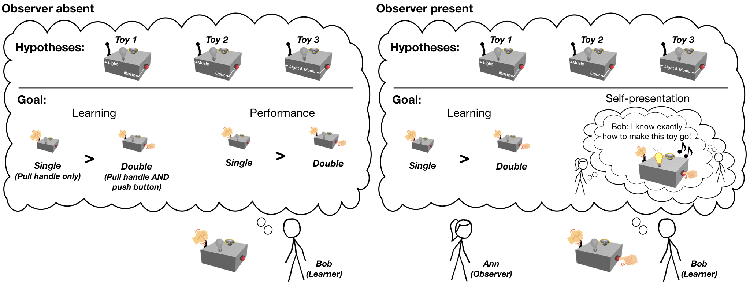
\includegraphics[width=1\linewidth]{figs/model_diagram-1} 

}

\caption[Diagram of the computational model]{Diagram of the computational model: The learner considers possible hypotheses and his contextual goals. When an observer is absent, he considers his learning goal (to maximize information gain) and performance goal (e.g. to play music) and decides on an action. When an observer is present, his decision for an action is based on his learning goal vs. presentational goal (to have the observer infer his competence).}\label{fig:model_diagram}
\end{figure*}
\end{CodeChunk}

But how can we begin to understand the role of \emph{social} factors in
self-directed learning contexts? Answering this question represents a
significant step because explore-exploit decisions often unfold within
fundamentally social contexts where people must integrate the value of
social goals and information goals when deciding what to do next.
Consider that actions that maximize learning are inherently risky --
leading to mistakes and struggles -- which could be difficult to
undertake in with someone else present. Thus, a learner might prioritize
actions that maintain their reputation: looking more attractive,
knowledgeable, or competent to the observer. In this case, the learner
is leveraging psychological reasoning processes to infer what the
observer thinks based on their action (cook a meal) and its outcome (a
delicious meal). If the learner is worried about the observer's beliefs,
then the they might choose actions that maximize the probability of
maintaining a favorable impression in the eyes of the observer (`That
meal was delicious, so he must be a good cook!'). Indeed, when the value
of self-presentation is highlighted, children avoid opportunities that
will help them learn new things but pose risks for public mistakes
(Dweck \& Leggett, 1988; Elliott \& Dweck, 1988).

We present the first computational model of the learning-performance
tradeoff in a self-directed learning context with social factors. We
model a learner who considers his learning goal versus performance goal,
which may be influenced by the social context (e.g.~the presence of
another individual whom he wants to impress). We then look at adult
participants' action choices within a minimalistic self-directed
learning task representing different goals and social contexts, and show
that people's choices are consistent with predictions of our model.

\section{Computational model}\label{computational-model}

To start to examine people's exploration-exploitation tradeoff, we
situate the model and paradigm in a simplistic learning environment. The
learner in our model is to act on a toy, and can choose between two
kinds of actions that will each lead to one outcome (new discovery) or
the other (overt reward). The learner's action rests on his goals to
explore versus exploit, and is determined in part by the presence or
absence of another person he cares about (i.e.~his
boss)\footnote{From here on, we use a male pronoun for Bob, the learner, and female pronoun for Ann, the boss and observer.}.

A key assumption underlying inferences in recent Bayesian models of
human social cognition is that people act approximately optimally given
a utility function (e.g. Goodman \& Frank, 2016; Jara-Ettinger, Gweon,
Schulz, \& Tenenbaum, 2016). Our model adopts the same utility-theoretic
approach, and assumes an approximately optimal agent, who reasons about
the utility function that represents a combination of multiple goals. In
a recent model of polite language production (Yoon, Tessler, Goodman, \&
Frank, 2017), the utility function comprised a weighted combination of
multiple utilities (goals) considered by the speaker, reflecting a
principled tradeoff between different communicative goals (e.g.~to be
informative, to be kind, and to appear to be a helpful speaker). We use
a similarly structured utility function that reflects different goals
that a learner has in a social learning context. Specifically, we model
how a person may make a decision to act based on his desire to learn how
a toy works (\emph{learning utility}), to make the toy operate and
perform a given function (\emph{performance utility}), or to present
himself as a competent individual who knows how to make the toy work
(\emph{presentational utility}; see the model diagram in Figure 1).

First, the \emph{learning utility} symbolizes the goal to learn new
information, which in our paradigm specifically is associated with
figuring out how a given toy works. The learning utility is formally
represented by an OED model (Lindley, 1956; ``Optimal Experiment
Design''; Nelson, 2005), which quantifies the \emph{expected utility} of
different information seeking actions. Here we follow the mathematical
details of the OED approach as outlined in Coenen, Nelson, \& Gureckis
(2017) that was implemented in our model. The set of queries, each
realized through taking an action, is defined as
\(Q_1, Q_2, ..., Q_n = {Q}\). The expected utility of each query
(\(EU(Q)\)) is a function of two factors: (1) the probability of
obtaining a specific answer \(P(a)\) weighted by (2) the usefulness of
that answer for achieving the learning goal \(U(a)\).

\[EU(Q) = \sum_{a\in q}{P(a)U(a)}\]

There are a variety of ways to define the usefulness function to score
each answer (for a detailed analysis of different approaches, see Nelson
(2005)). One standard method is to use \emph{information gain}, which is
defined as the change in the learner's overall uncertainty (difference
in entropy) before and after receiving an answer. This information gain
is then the usefulness of the answer to the query, and thus is equal to
the learning utility:

\[ U_{learning} = U(a) = ent(H) - ent(H|a)\] \noindent
where \(ent(H)\) is defined using Shannon
entropy\footnote{Shannon entropy is a measure of unpredictability or amount of uncertainty in the learner's probability distribution over hypotheses. Intuitively, higher entropy distributions are more uncertain and harder to predict. For example, if the learner believes that all hypotheses are equally likely, then they are in a state of high uncertainty/entropy. In contrast, if the learner firmly believes in one hypothesis, then uncertainty/entropy is low.}.
MacKay (2003), which provides a measure of the overall amount of
uncertainty in the learner's beliefs about the candidate hypotheses.

\[ent(H) = -\sum_{a\in A}{P(h)log_2P(h)}\] \noindent
The conditional entropy computation is the same, but takes into account
the change in the learner's beliefs after seeing an answer.

\[ ent(H|a) = -\sum_{h\in H}{P(h|a)logP(h|a)} \] \noindent
To calculate the change in the learner's belief in a hypothesis
\(P(h|a)\), we use Bayes rule.

\[ P(h|a) = \frac{P(h)P(a|h)}{P(a)} \]

\noindent
The learner performs the expected utility computation for each query in
the set of possible queries and picks the one that maximizes utility. In
practice, the learner considers each possible answer, scores the answer
with the usefulness function, and weights the score using the
probability of getting that answer. In our paradigm, a learner thinking
about the learning utility considers acting on the toy one way over
another, and computes how informative a given answer should be in
reducing uncertainty about how the toy works.

Second, the \emph{performance utility} is the utility of successfully
making the toy operate. Specifically within our current paradigm, the
performance utility is the expected utility of music playing (\(m\))
given the learner's action \(a\).

\[ U_{performance} = P_L(m | a) \] \noindent
Thus, performance utility is maximized by taking an action that is most
likely to make the toy ``go'' and play music, which is the operation of
interest.

When there is no observer present, the learner considers the tradeoff
between the learning utility and performance utility, and he determines
his action based on a weighted combination of the two utilities:

\[ U(a;\phi; obs = no) = \phi \cdot U_{learning} + (1-\phi) \cdot U_{performance} ,\]
\noindent
where \(\phi\) is a mixture parameter governing the extent to which the
learner prioritizes information gain over making the toy play music.

When there is another person present to observe the learner's action,
this observer \(O\) reasons about the competence \(c\) of the learner
\(L\) which is equal to whether the learner was able to make the toy
work.

\[ P_O(c) \propto P_L(m | a)\]

The learner thinks about how the observer infers the learner's
competence, and his \emph{presentational} utility is based on maximizing
the apparent competence inferred by the observer.

\[ U_{presentation} = P_O(c) \] Thus, when there is an observer present,
the learner considers the tradeoff between the learning utility and
presentational utility:

\[ U(m;a;\phi; obs = yes) = \phi \cdot U_{learning} + (1-\phi) \cdot U_{presentational}\]
Based on the utility functions above, the learner (\(L\)) chooses his
action \(a\) approximately optimally (as per optimality parameter
\(\lambda\)) given his goal weight and observer presence.

\[ P_L(a | \phi, obs) \propto \exp(\lambda \cdot \mathbb{E}[U(a;\phi; obs)])\]

\section{Experiment 1}\label{experiment-1}

\begin{CodeChunk}
\begin{figure*}[t]

{\centering 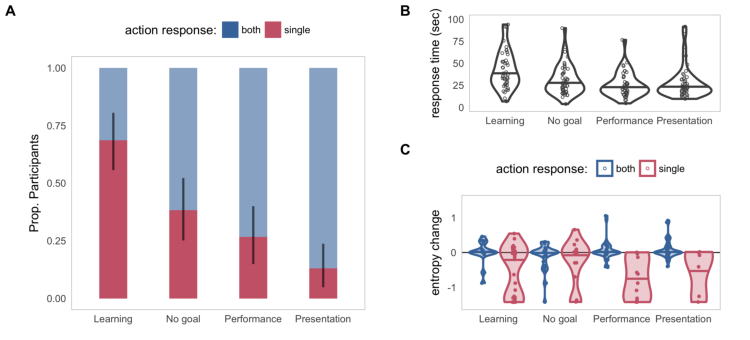
\includegraphics[width=0.95\linewidth]{figs/e1_behav_results-1} 

}

\caption[Behavioral results for E1]{Behavioral results for E1.}\label{fig:e1_behav_results}
\end{figure*}
\end{CodeChunk}

In our Experiments, we wanted to look at people's action choices in a
minimalistic self-directed learning environment with varying goals and
social contexts. In Experiment 1, we wanted to confirm that participants
will choose actions based on different goal descriptions, depending on
whether we highlight learning goal, performance goal, or presentation
goal.

We were interested to see what people will choose to do when no goal is
specified and they are free to explore. Thus, we asked participants to
imagine a scenario in which they were expected to act on a toy with an
uncertain causal mechanism, and we assigned participants to different
goal conditions: learning goal (i.e.~learn how the toy works);
performance goal (e.g.~make the toy play music); presentation goal
(i.e.~impress their boss); and no goal.

\subsection{Method}\label{method}

\subsubsection{Participants}\label{participants}

FIXME participants with IP addresses in the United States were recruited
on Amazon's Mechanical Turk. We excluded FIXME partcipants who failed to
answer at least two out of three set of manipulation check questions
correctly (See Procedure section for details on the manipulation check
questions), and thus the remaining FIXME participants were included in
our final analysis.

\subsubsection{Stimuli and Design}\label{stimuli-and-design}

We presented images of three different toys that look very similar but
each work in different ways, and provided instructions for them (see top
of Fig. 1 for the toy types). Toy 1 instructions were: \emph{``Pull the
handle on the left to turn on the light.Press the button on the right to
play music. Doing both produces both effects at the same time.''} Toy 2
instuctions were: \emph{``Pull the handle on the left to play music.
Press the button on the right to turn on the light. Doing both produces
both effects.''} Toy 3 instuctions were: \emph{``Pull the handle on the
left AND press the button on the right to turn on the light and play
music at the same time. The button press or handle pull on its own
doesn't produce any effect.''} Each toy had a label at the front,
indicating which action(s) will make the toy operate, and with which
outcome effect.

We asked participants to act on one of these toys; importantly, the
given toy was missing its label, such that partcipants could not know
whether the toy was Toy 1, 2 or 3. We assigned participants into four
goal conditions: For participants in \emph{learning},
\emph{performance}, and \emph{presentation} conditions, we asked them to
imagine that they were children's toy developers and that one day, their
boss approached them and said: ``That must be one of the new toys that
you've been working on. But it looks like you forgot to put on the
label! Can you figure out whether this toy is a ButtonMusic toy,
HandleMusic toy, or BothMusicLight toy?'' (\emph{learning} condition);
``That must be one of the new toys that you've been working on. I want
to hear the music it plays.'' (\emph{performance} condition); or ``That
must be one of the new toys that you've been working on. How does it
work?'' followed by the prompt ``\ldots{} {[}Imagine{]} you only had one
chance to impress your boss and show that you're competent \ldots{}''
(\emph{presentation} condition). We asked participants to select an
action they would like to try out on the toy in order to accomplish the
specified goal, out of three possible actions: to ``press the button'',
``pull the handle'', or ``press the button and pull the handle.'' We
randomly assigned each participant to one of the three goal conditions,
and randomized the order of actions to choose from.

\subsubsection{Procedure}\label{procedure}

We first introduced participants to the task, by asking them to
``Imagine that {[}they{]} are a children's toy developer, and
{[}they've{]} designed three toys that each work in different ways''. We
showed them a picture of a possible toy with labels on its different
parts. Then they read instructions for each of the three toy types. We
presented Toy 1 and Toy 2 instructions in a randomized order first, and
then Toy 3 instructions. Afterwards, they were asked what they would do
to make the toy operate as manipulation check (e.g. ``How would you make
the toy play music?''). We asked participants to rate prior likelihood
that an unknown toy is a ButtonMusic toy, HandleMusic toy, or
BothMusicLight toy, to use as priors for our model. Participants then
read a scenario for one of the three goal conditions, followed by the
question: ``If you only had one chance to try a SINGLE action to
{[}goal{]}, which action would you want to take? You will get a 10 cent
bonus after submitting the HIT if you {[}goal{]}.'' After selecting one
of three possible actions to perform on the toy and seeing that the toy
successfully played music, participants were asked again to rate the
likelihood that the unlabeled toy was each of the three possible toys.
Our hypothesis and method were pre-registered prior to data collection
on the Open Science Framework (\url{https://osf.io/kcjau}).

\subsection{Results and discussion}\label{results-and-discussion}

\subsubsection{Action selections}\label{action-selections}

\subsubsection{Action response times}\label{action-response-times}

\subsubsection{Belief change}\label{belief-change}

\subsubsection{BDA model-data fits}\label{bda-model-data-fits}

\section{Experiment 2}\label{experiment-2}

\begin{CodeChunk}
\begin{figure*}[t]

{\centering 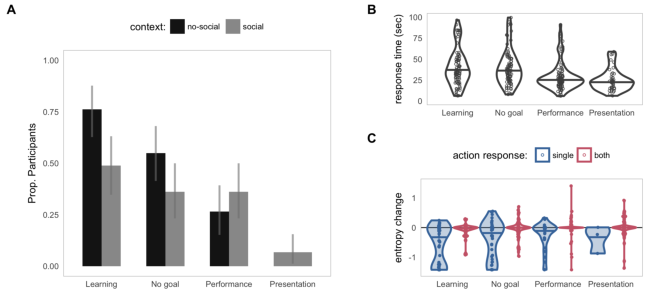
\includegraphics[width=0.95\linewidth]{figs/e2_behav_results-1} 

}

\caption[Behavioral results for E2]{Behavioral results for E2.}\label{fig:e2_behav_results}
\end{figure*}
\end{CodeChunk}

\subsection{Method}\label{method-1}

\subsubsection{Participants}\label{participants-1}

\subsubsection{Stimuli and design}\label{stimuli-and-design-1}

\subsubsection{Procedure}\label{procedure-1}

\subsection{Results and discussion}\label{results-and-discussion-1}

\subsubsection{Action selections}\label{action-selections-1}

\subsubsection{Action response times}\label{action-response-times-1}

\subsubsection{Belief change}\label{belief-change-1}

\subsubsection{BDA model-data fits}\label{bda-model-data-fits-1}

\section{General Discussion}\label{general-discussion}

\section{Acknowledgements}\label{acknowledgements}

This work was supported by NSERC postgraduate doctoral scholarship
PGSD3-454094-2014 to EJY and an NSF GRFP to KM {[}FIXME{]}.

\section{References}\label{references}

\setlength{\parindent}{-0.1in} \setlength{\leftskip}{0.125in} \noindent

\hypertarget{refs}{}
\hypertarget{ref-castro2009human}{}
Castro, R. M., Kalish, C., Nowak, R., Qian, R., Rogers, T., \& Zhu, X.
(2009). Human active learning. In \emph{Advances in neural information
processing systems} (pp. 241--248).

\hypertarget{ref-chi2009active}{}
Chi, M. T. (2009). Active-constructive-interactive: A conceptual
framework for differentiating learning activities. \emph{Topics in
Cognitive Science}, \emph{1}(1), 73--105.

\hypertarget{ref-coenen2017}{}
Coenen, A., Nelson, J. D., \& Gureckis, T. M. (2017). Asking the right
questions about human inquiry.

\hypertarget{ref-dweck1988}{}
Dweck, C. S., \& Leggett, E. L. (1988). A social-cognitive approach to
motivation and personality. \emph{Psychological Review}, \emph{95}(2),
256.

\hypertarget{ref-elliott1988}{}
Elliott, E. S., \& Dweck, C. S. (1988). Goals: An approach to motivation
and achievement. \emph{Journal of Personality and Social Psychology},
\emph{54}(1), 5.

\hypertarget{ref-goodman2016}{}
Goodman, N. D., \& Frank, M. C. (2016). Pragmatic language
interpretation as probabilistic inference. \emph{Trends in Cognitive
Sciences}, \emph{20}(11), 818--829.

\hypertarget{ref-grabinger1995rich}{}
Grabinger, R. S., \& Dunlap, J. C. (1995). Rich environments for active
learning: A definition. \emph{ALT-J}, \emph{3}(2), 5--34.

\hypertarget{ref-jara2016}{}
Jara-Ettinger, J., Gweon, H., Schulz, L. E., \& Tenenbaum, J. B. (2016).
The naïve utility calculus: Computational principles underlying
commonsense psychology. \emph{Trends in Cognitive Sciences},
\emph{20}(8), 589--604.

\hypertarget{ref-lindley1956}{}
Lindley, D. V. (1956). On a measure of the information provided by an
experiment. \emph{The Annals of Mathematical Statistics}, 986--1005.

\hypertarget{ref-mackay2003}{}
MacKay, D. J. (2003). \emph{Information theory, inference and learning
algorithms}. Cambridge university press.

\hypertarget{ref-nelson2005}{}
Nelson, J. D. (2005). Finding useful questions: On bayesian
diagnosticity, probability, impact, and information gain.
\emph{Psychological Review}, \emph{112}(4).

\hypertarget{ref-prince2004does}{}
Prince, M. (2004). Does active learning work? A review of the research.
\emph{Journal of Engineering Education}, \emph{93}(3), 223--231.

\hypertarget{ref-ramirez2017active}{}
Ramirez-Loaiza, M. E., Sharma, M., Kumar, G., \& Bilgic, M. (2017).
Active learning: An empirical study of common baselines. \emph{Data
Mining and Knowledge Discovery}, \emph{31}(2), 287--313.

\hypertarget{ref-settles2012active}{}
Settles, B. (2012). Active learning. \emph{Synthesis Lectures on
Artificial Intelligence and Machine Learning}, \emph{6}(1), 1--114.

\hypertarget{ref-shafto2012learning}{}
Shafto, P., Goodman, N. D., \& Frank, M. C. (2012). Learning from
others: The consequences of psychological reasoning for human learning.
\emph{Perspectives on Psychological Science}, \emph{7}(4), 341--351.

\hypertarget{ref-sutton1998}{}
Sutton, R. S., \& Barto, A. G. (1998). \emph{Introduction to
reinforcement learning} (Vol. 135). MIT Press Cambridge.

\hypertarget{ref-yoon2017}{}
Yoon, E. J., Tessler, M. H., Goodman, N. D., \& Frank, M. C. (2017). ``I
won't lie, it wasn't amazing'': Modeling polite indirect speech. In
\emph{Proceedings of the thirty-ninth annual conference of the Cognitive
Science Society}.

\end{document}
